\documentclass[11pt]{article}
\usepackage[a4paper,margin=1in]{geometry}
\usepackage{amsmath,amssymb,amsthm,mathtools}
\usepackage{booktabs}
\usepackage{enumitem}
\usepackage{graphicx}
\usepackage{microtype}
\usepackage{hyperref}
\usepackage[nameinlink,capitalise]{cleveref}
\usepackage[numbers,sort&compress]{natbib}

\newtheorem{theorem}{Theorem}[section]
\newtheorem{proposition}[theorem]{Proposition}
\newtheorem{corollary}[theorem]{Corollary}
\theoremstyle{definition}
\newtheorem{definition}[theorem]{Definition}
\theoremstyle{remark}
\newtheorem{remark}[theorem]{Remark}
\newcommand{\norm}[1]{\left\lVert#1\right\rVert}

\title{An Explicit Sigma-Power Ledger for Prefix and Observability Bridges\\
\large Max-Plus Composition and Two Independence Barriers}
\author{Liang Wang}
\date{July 2026}

\begin{document}
\maketitle

\begin{abstract}
RH-101 removes ambient Gram assembly from the recursive packet route and
RH-102 supplies an exact stopped endpoint budget.  The remaining inherited
gate was described only as a ``prefix/normalization/observability bridge.''
We replace that phrase by an exact sigma-power ledger and determine what the
normalized packet mechanics can and cannot imply.

For one directional Hardy triple, write the source as
$X_\sigma=N_\sigma\bar X_\sigma$, split at a block horizon $M_\sigma$, let
$P_\sigma$ be the unit-source finite-prefix norm, $Z_\sigma$ the reduced
packet future, $R_\sigma$ the postblock packet residual, $\Omega_\sigma$ the
future observability factor, and $U_\sigma$ an upstream Hardy bridge.  Exact
prefix/future decomposition and the RH-77 observability theorem give
\[
 \mathcal E_\sigma
 \le U_\sigma+N_\sigma
 \bigl(P_\sigma+Z_\sigma+\Omega_\sigma R_\sigma\bigr).
\]
If a signed power $a(f)$ means
$f=O(\sigma^{-a(f)}\operatorname{polylog}(1/\sigma))$, then the directional
Hardy growth power is
\[
 \alpha_s=max\{0,u_s,n_s+p_s,n_s+z_s,n_s+o_s+r_s\}.
\]
The two directions add:
$\delta=\alpha_L+\alpha_R$.  The inherited RH-49 full strict-mesh range is
available when $\delta\le1/4$, while on
$n=\sigma^{-2}L(\sigma)$ the displayed RH-54 envelope has decay power
$3/4-\delta$.

This ledger closes several bookkeeping questions.  Coupling normalization,
logarithmic packet rank, depth-five memory, the fixed stopped gate, and mesh
substitution all carry zero sigma power.  Observation growth may be cancelled
by residual decay because $o_s+r_s$ is a signed sum; terms within one direction
combine by a maximum, not by addition.

It also gives a negative theorem.  A nilpotent two-dimensional family has
normalized packet Gram equal to one and zero postblock tail, yet finite-prefix
Hardy power equal to any prescribed $a>0$.  A scalar stable family likewise
has a perfect rank-one packet at every time while observation scaling creates
any prescribed Hardy power $b>0$.  Thus a uniform quotient law, structured
Gram action, and stopped clock cannot by themselves prove the prefix or
absolute observability estimates.

The five-anchor ledger remains fully green: conditional Hardy uppers are at
most $1.836$, rank clocks are at most seven, depth five and the stopped
$1.01$ gate persist, and the stress identification envelope decreases from
$0.07354$ to $0.002961$.  These finite facts do not close the new all-level
scalar leaves.  Hence the optimistic claim that only the quotient gate
remains must be revised.  No unconditional Stage A, moving-cloud
construction, Hilbert--Polya operator, zero identification, or Riemann
Hypothesis result is claimed.
\end{abstract}

\noindent\textbf{Keywords:} sigma-power ledger; max-plus algebra; Hardy
energy; observability Gramian; normalized packet; finite-prefix transient.

\medskip
\noindent\textbf{MSC 2020:} 47A55; 93B28; 65F15; 37M25; 15A18.

\section{Introduction}

The packet corridor now has unusually explicit finite-dimensional mechanics.
Source-seeded refresh avoids late ambient eigenspaces, reduced moments avoid
ambient cross factorizations, finite-memory state actions avoid ambient
Gramians, and an exact stopped clock prevents locally certified quotients from
overspending the endpoint gate
\citep{WangSourceSeeded2026,WangFiniteMemory2026,WangStoppedClock2026}.
These are genuine advances, but they concern relative packet geometry.

Stage A ultimately needs an absolute directional Hardy norm.  The RH-100
route review retained a separate gate $O$ for finite prefix, normalization,
and observability, then proposed RH-103 to expose its powers rather than hide
them under ``polylogarithmic'' \citep{WangHundredLayer2026}.  That distinction
is essential: normalization can erase a scalar amplitude from every packet
Gramian, while the same amplitude still appears in an unnormalized transfer
sequence or observation.

This paper has two goals.  First, it proves the exact max-plus sigma-power
formula for the effective-rank corridor.  Second, it tests whether the packet
gates can imply the missing terms.  Two elementary stable families show that
they cannot.  The result is not a failure of the packet route; it is a sharper
dependency graph.  The remaining wall consists of explicit scalar exponent
laws that can be attacked separately.

\section{Directional prefix/future decomposition}
\label{sec:decomposition}

Let $A_\sigma\in\mathbb C^{d\times d}$, source $X_\sigma$, and observation
$Y_\sigma$.  The directional Hardy norm is
\begin{equation}
 \mathcal E_\sigma^2
 =\sum_{j\ge0}\norm{Y_\sigma A_\sigma^jX_\sigma}_F^2.
 \label{eq:hardy}
\end{equation}
Write
\[
 X_\sigma=N_\sigma\bar X_\sigma,
 \qquad \norm{\bar X_\sigma}_F=1,
\]
where $N_\sigma$ includes the actual normalized coupling/range factor used by
the physical triple.  At a block horizon $M=M_\sigma$, define
\begin{align}
 P_\sigma^2
 &=\sum_{j=0}^{M-1}
   \norm{Y_\sigma A_\sigma^j\bar X_\sigma}_F^2,
 \label{eq:prefix}\\
 \bar B_\sigma&=A_\sigma^M\bar X_\sigma.
\end{align}
Let $\bar B_{\sigma,r}$ be a rank-$r$ approximation and put
\begin{align}
 Z_\sigma&=T_\sigma(\bar B_{\sigma,r}),\label{eq:reduced}\\
 R_\sigma&=\norm{\bar B_\sigma-\bar B_{\sigma,r}}_F.
 \label{eq:residual}
\end{align}
Here $T_\sigma$ is the complete future Hardy seminorm.  If
$q_\sigma=\norm{A_\sigma^M}_2<1$, the RH-77 block-observability theorem gives
\begin{equation}
 \Omega_\sigma=
 \sqrt{\frac{\norm{O_{\sigma,M}}_2}{1-q_\sigma^2}},
 \qquad
 |T_\sigma(\bar B_\sigma)-Z_\sigma|
 \le\Omega_\sigma R_\sigma.
 \label{eq:observability}
\end{equation}

Finally, let $U_\sigma$ be a Hardy-norm upper for the analytic/frozen or
upstream/reference transfer difference.  RH-74 constructs this object at the
five anchors \citep{WangUpstream2026}.

\begin{theorem}[Explicit prefix--packet--observability ledger]
\label{thm:norm-ledger}
The complete directional norm satisfies
\begin{equation}
 \boxed{
 \mathcal E_\sigma
 \le U_\sigma+N_\sigma
 \bigl(P_\sigma+Z_\sigma+\Omega_\sigma R_\sigma\bigr).}
 \label{eq:norm-ledger}
\end{equation}
\end{theorem}

\begin{proof}
The triangle inequality separates the upstream/reference bridge.  For the
reference triple, split \eqref{eq:hardy} before and after $M$.  The finite
part is $N_\sigma P_\sigma$.  Apply the reverse triangle inequality for the
future seminorm and \eqref{eq:observability} to obtain
$N_\sigma(Z_\sigma+\Omega_\sigma R_\sigma)$.
\end{proof}

The theorem deliberately keeps the observability factor and residual
separate.  One may grow while the other decays.  Multiplying two separately
fitted absolute powers only after their signs are recorded prevents a common
bookkeeping error.

\section{Signed sigma powers and max-plus composition}
\label{sec:powers}

\begin{definition}[Signed sigma power]
For a nonnegative family $f_\sigma$, a signed ledger power $a_f\in\mathbb R$
means
\[
 f_\sigma
 =O\!\left(\sigma^{-a_f}
 \operatorname{polylog}(1/\sigma)\right).
\]
A negative $a_f$ records decay.  The final Hardy growth exponent is truncated
below at zero.
\end{definition}

Let $u_s,n_s,p_s,z_s,o_s,r_s$ be the powers of the six terms in
\eqref{eq:norm-ledger} for side $s\in\{L,R\}$.

\begin{theorem}[Max-plus directional Hardy power theorem]
\label{thm:power-ledger}
The directional growth power may be chosen as
\begin{equation}
 \boxed{
 \alpha_s=max\{0,u_s,n_s+p_s,n_s+z_s,n_s+o_s+r_s\}.}
 \label{eq:alpha}
\end{equation}
For the RH-54 two-sided composition,
\begin{equation}
 \delta=\alpha_L+\alpha_R,
 \qquad
 \norm{\mathcal I_{n,\sigma}}_{S_2}
 =O\!\left(n^{-2}\sigma^{-13/4-\delta}
 \operatorname{polylog}(1/\sigma)\right).
 \label{eq:identification}
\end{equation}
The inherited RH-49 full strict-mesh range is green when
\begin{equation}
 \delta\le\frac14.
 \label{eq:quarter}
\end{equation}
On the displayed stress schedule
$n=\sigma^{-2}L(\sigma)$, the envelope in
\eqref{eq:identification} has sigma decay power
\begin{equation}
 \frac34-\delta.
 \label{eq:stress}
\end{equation}
\end{theorem}

\begin{proof}
Products add signed powers and finite sums take their maximum.  Apply those
two rules to \eqref{eq:norm-ledger}, including zero because a bounded Hardy
norm has growth power zero.  RH-54 proves that the two directional powers add
in the Hilbert--Schmidt gain and yields \eqref{eq:identification}
\citep{WangFactorAware2026}.  The RH-49 stable-rank threshold is
\eqref{eq:quarter}.  Substituting $n=\sigma^{-2}L(\sigma)$ gives
\eqref{eq:stress}.
\end{proof}

\begin{remark}
Terms within one side take a maximum, not a sum.  Prefix growth and reduced
future growth are alternative contributions to the same norm.  By contrast,
the left and right Hardy powers add because the downstream directional gain
contains their product.
\end{remark}

\begin{remark}
The stress exponent can remain positive when $\delta>1/4$.  That does not
override the established RH-49 claim boundary: the quarter-power condition is
the sufficient threshold for retaining the full strict mesh range, not merely
one chosen stress schedule.
\end{remark}

\section{Zero-power overheads already closed}
\label{sec:zero}

Several quantities in the packet architecture do not consume the quarter
budget.
\begin{enumerate}[leftmargin=2em]
\item The couplings $B$ and $C$ are normalized in Hilbert--Schmidt norm.
RH-52 bounds the required range-restricted residues, and RH-54 proves that
normalization converts the adaptive cutoff defect into a decaying relative
error.  Thus $n_s=0$ in the intended ledger
\citep{WangFactorTransfer2026,WangFactorAware2026}.
\item The half-logarithmic rank $r_\sigma=O(\log(1/\sigma))$ carries zero
sigma power \citep{WangHalfLog2026}.
\item The RH-101 common memory depth is five and $\eta=1/512$, both constants.
\item The RH-102 target $1.01$ and safety fraction $0.99$ are constants.
\item Replacing $n$ by $\sigma^{-2}L(\sigma)$ is exact algebra; logarithmic
$L$ does not create a sigma power.
\end{enumerate}

These facts are useful, but they do not bound $P_\sigma$, $Z_\sigma$, or
$\Omega_\sigma R_\sigma$.

\section{Two independence barriers}
\label{sec:barriers}

The next propositions show that the missing terms cannot be recovered from
perfect normalized packets alone.

\begin{proposition}[Finite-prefix independence barrier]
\label{prop:prefix-barrier}
For every $a>0$, let
\[
 A_\sigma=
 \begin{pmatrix}0&\sigma^{-a}\\0&0\end{pmatrix},
 \qquad X=e_2,qquad Y=e_1^*.
\]
Then $A_\sigma^2=0$ and
\begin{equation}
 \mathcal E_\sigma=\sigma^{-a}.
 \label{eq:prefix-example}
\end{equation}
Every nonzero state has one source coordinate, so its normalized packet
Gramian is the scalar $1$ and its rank-one relative tail is zero.  The
postblock future after two steps is also zero.
\end{proposition}

\begin{proof}
$YX=0$, $YA_\sigma X=\sigma^{-a}$, and all later responses vanish.  This
gives \eqref{eq:prefix-example}.  A nonzero one-column state $S$ satisfies
$S^*S/\norm S_F^2=[1]$, so normalized packet data contain no trace of the
transient amplitude.
\end{proof}

\begin{proposition}[Observation independence barrier]
\label{prop:observation-barrier}
For every $b>0$, take the scalar stable system
\[
 A=c,qquad X=1,qquad Y_\sigma=\sigma^{-b},qquad 0<c<1.
\]
Every normalized state Gramian is $1$ and every rank-one packet tail is zero,
while
\begin{equation}
 \mathcal E_\sigma
 =\frac{\sigma^{-b}}{\sqrt{1-c^2}}.
 \label{eq:observation-example}
\end{equation}
\end{proposition}

\begin{proof}
The packet statement is immediate in one dimension.  Summing the scalar
geometric Hardy series gives \eqref{eq:observation-example}.
\end{proof}

Both systems are stable; the first is nilpotent.  The propositions do not say
that the physical folded-Gaussian family has these bad powers.  They prove a
logical separation: $Q$, $G$, and $H_{\rm stop}$ cannot imply the missing
prefix and observation laws without additional physical input.

\section{Five-anchor ledger}
\label{sec:audit}

The machine-readable audit combines RH-74, RH-75, RH-77, RH-78, RH-82,
RH-101, and RH-102 without refitting an all-level law.  Selected quantities
are shown in \cref{tab:anchors}.

\begin{table}[t]
\centering
\caption{Finite-anchor quantities.  The observed residual product already
includes future observability; its small size does not bound either factor
uniformly.}
\label{tab:anchors}
\begin{tabular}{@{}rrrrrrr@{}}
\toprule
$\sigma$ & prefix & $\norm O^{1/2}$ & observed residual & bridge & rank & Hardy\\
\midrule
0.16 & 1.003 & 4.097  & $5.04\,10^{-9}$  & $1.42\,10^{-6}$ & 4 & 1.078\\
0.08 & 1.265 & 6.076  & $2.11\,10^{-12}$ & $8.13\,10^{-7}$ & 5 & 1.309\\
0.04 & 1.485 & 9.299  & $7.26\,10^{-13}$ & $2.02\,10^{-6}$ & 6 & 1.506\\
0.02 & 1.634 & 14.099 & $6.26\,10^{-12}$ & $6.63\,10^{-7}$ & 6 & 1.679\\
0.01 & 1.760 & 21.255 & $1.75\,10^{-12}$ & $3.12\,10^{-7}$ & 7 & 1.836\\
\bottomrule
\end{tabular}
\end{table}

The absolute observability factor grows from $4.10$ to $21.26$, while the
observation-weighted clock residual remains below $5.05\times10^{-9}$.  This
is precisely why the signed sum $o_s+r_s$ is the correct ledger entry.  A
separate theorem must show that the residual decay compensates observation
growth at every level.

The depth-five action passes, the primary stopped endpoint ratio is at most
$1.00117243$, and every finite anchor remains inside the conditional
zero-power Hardy envelope.  On the RH-78 stress mesh, the archived
identification envelope decreases from $0.07354$ to $0.002961$.

\begin{table}[t]
\centering
\caption{Illustrative exact max-plus scenarios.  These are power allocations,
not fits to the physical family.}
\label{tab:scenarios}
\begin{tabular}{@{}lrrrr@{}}
\toprule
scenario & $\alpha_L$ & $\alpha_R$ & $\delta$ & quarter gate\\
\midrule
zero-power target & 0 & 0 & 0 & green\\
balanced boundary & 0.125 & 0.125 & 0.25 & green\\
one-sided observation leak & 0.30 & 0 & 0.30 & red\\
two-sided prefix leak & 0.16 & 0.12 & 0.28 & red\\
observation/residual cancellation & 0 & 0 & 0 & green\\
max-not-sum example & 0.12 & 0.10 & 0.22 & green\\
\bottomrule
\end{tabular}
\end{table}

\begin{figure}[t]
\centering
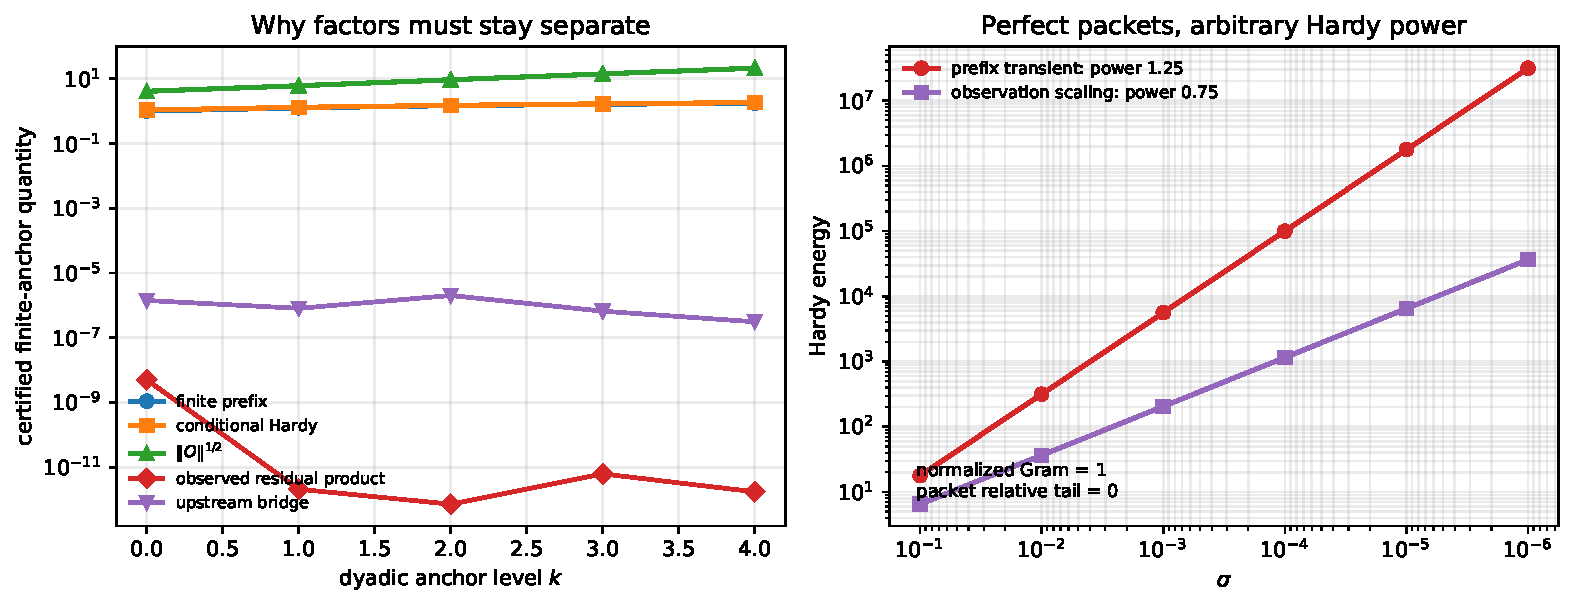
\includegraphics[width=\textwidth]{figures/prefix_observability_power_ledger.pdf}
\caption{Left: finite factors have very different scales and must remain
separate in the asymptotic ledger.  Right: two exact stable families keep
normalized packet tails zero while assigning arbitrary Hardy powers.}
\label{fig:ledger}
\end{figure}

\section{Revised Stage-A frontier}
\label{sec:route}

The RH-100 optimistic branch said that positive RH-101--RH-103 results could
leave only the uniform quotient law $Q$.  RH-101 and RH-102 are positive in
their stated scopes.  RH-103 is mixed:
\begin{itemize}[leftmargin=2em]
\item normalization, rank, memory, stopping, and mesh bookkeeping are closed
at zero sigma power;
\item the exact exponent formula is closed;
\item the five-anchor composition is green;
\item the all-level prefix and absolute observation-weighted future laws are
logically independent of normalized packet success.
\end{itemize}

Therefore $O$ must not be deleted.  It should be replaced by named scalar
leaves corresponding to $u_s$, $p_s$, $z_s$, and $o_s+r_s$.  Some future
formulation of $Q$ may also provide part of $r_s$; it still cannot provide
$p_s$ or $o_s$ by itself, as \cref{prop:prefix-barrier,prop:observation-barrier}
show.

The fallback RH-75 full-block law remains valid: its square-root contraction
explicitly supplies the observation/residual cancellation together with a
finite-prefix companion.  The packet route remains attractive because it can
attack weaker directional terms, but it now has a more honest list of them.

No unconditional Stage A follows from this ledger.  Moving-cloud Riesz
projections, coefficient bridges, trace-class complements, self-adjoint
counting, arithmetic trace formulas, and zero identification remain
downstream.  In particular, no Hilbert--Polya operator or proof of the
Riemann Hypothesis is claimed.

\section{Conclusion}

The word ``polylogarithmic'' has been replaced by an exact max-plus formula.
Within one directional Hardy norm, alternative contributions take a maximum;
observation and residual powers add with sign; the two directions then add
against one shared quarter-power budget.  Several packet overheads cost no
sigma power at all.

The same analysis prevents an overclaim.  Perfect normalized packets do not
bound finite transients or absolute observation scale.  The next subprogram
should therefore prove a physical finite-prefix law and an
observation--residual cancellation law, while continuing the uniform
gap-aware quotient attack.  That is a narrower and more testable frontier
than the former single letter $O$.

\bibliographystyle{plainnat}
\bibliography{references}

\end{document}
